%===============================================================================
% $Id: ifacconf.tex 7 2007-11-21 12:50:23Z jpuente $
% Template for IFAC meeting papers
% Copyright (c) 2007 International Federation of Automatic Control
%===============================================================================
\documentclass{ifacconf}
\usepackage[round]{natbib} % you should have natbib.sty
\usepackage{graphicx}      % include this line if your document contains figures

\usepackage{amsmath,amssymb}
\usepackage{url}
\usepackage{diffcoeff}
\usepackage{bm}

\usepackage{mathrsfs}
\usepackage{multirow}

\usepackage{caption, subfig}

\usepackage{xcolor,colortbl}

\newcommand{\mc}[2]{\multicolumn{#1}{c}{#2}}
% normal box
\newcommand{\sqboxs}{1.2ex}% the square size
\newcommand{\sqboxf}{0.6pt}% the border in \sqboxEmpty
\newcommand{\sqbox}[1]{\textcolor{#1}{\rule{\sqboxs}{\sqboxs}}}

\definecolor{Blue}{rgb}{0,1,1}
\definecolor{Green}{rgb}{0.4,1,0.4}
\definecolor{GreenYellow}{rgb}{0.3,0.6,0.5}
\definecolor{Yellow}{rgb}{1,1,0.4}
\definecolor{Orange}{rgb}{1,0.6,0.2}
\definecolor{Purple}{rgb}{1,0.5,0.5}
\definecolor{Red}{rgb}{1,0.2,0.2}

\definecolor{Grey}{rgb}{0.5,0.5,0.5}


\newcolumntype{g}{>{\columncolor{Green}}c}
\newcolumntype{m}{>{\columncolor{Yellow}}c}
\newcolumntype{b}{>{\columncolor{Blue}}c}


\newtheorem{remark}{Remark}

\DeclareMathOperator*{\argmax}{arg\,max}
\DeclareMathOperator*{\argmin}{arg\,min}
\DeclareMathOperator{\Tr}{Tr}

\def\onedot{$\mathsurround0pt\ldotp$}
\def\cddot{% two dots stacked vertically
	\mathbin{\vcenter{\baselineskip.67ex
			\hbox{\onedot}\hbox{\onedot}}%
}}

\makeatletter \renewcommand\d[1]{\ensuremath{%
		\;\mathrm{d}#1\@ifnextchar\d{\!}{}}}
\makeatother

\bibliographystyle{agsm}
\graphicspath{{./Figures/}}
%===============================================================================
\begin{document}
\begin{frontmatter}

\title{Partitioned Finite Element Method for the Mindlin Plate as a Port-Hamiltonian system \thanksref{footnoteinfo}} 
% Title, preferably not more than 10 words.

\thanks[footnoteinfo]{This work is  supported by the project ANR-16-CE92-0028,
	entitled {\em Interconnected Infinite-Dimensional systems for Heterogeneous
		Media}, INFIDHEM, financed by the French National
	Research Agency (ANR) and the Deutsche Forschungsgemeinschaft (DFG). Further information is available at {\url{https://websites.isae-supaero.fr/infidhem/the-project}}.
	}

\author[ISAE]{Andrea Brugnoli}
\author[ISAE]{Daniel Alazard} 
\author[ISAE]{Val\'erie Pommier-Budinger}
\author[ISAE]{Denis Matignon}

\address[ISAE]{ISAE-SUPAERO, Universit\'e de Toulouse, France.\\
	10 Avenue Edouard Belin, BP-54032, 31055 Toulouse Cedex 4. \\
	Andrea.Brugnoli@isae.fr,  Daniel.Alazard@isae.fr, \\
	Valerie.Budinger@isae.fr, Denis.Matignon@isae.fr}

\begin{abstract}
The port-Hamiltonian framework allows for a structured representation and interconnection of distributed parameter systems described by Partial Differential Equations (PDE) from different realms. Here, the Mindlin-Reissner model of a thick plate is presented in a tensorial formulation. Taking into account collocated boundary control and observation gives rise to an infinite-dimensional port-Hamiltonian system (pHs). The Partitioned Finite Element Method (PFEM), already presented in our previous work, allows obtaining a structure-preserving finite-dimensional port-Hamiltonian system, and accounting for boundary control in a straightforward manner. In order to illustrate the flexibility of PFEM, both types of boundary controls can be dealt with: either through forces and momenta, or through kinematic variables. The discrete model is easily implementable by using the FEniCS platform. Computation of eigenfrequencies and vibration modes, together with time-domain simulation results demonstrate the consistency of the proposed approach.
\end{abstract}

\begin{keyword}
Port-Hamiltonian systems (pHs), Geometric Discretization, Mindlin-Reissner Plate, Partitioned Finite Element Method (PFEM), Symplectic Integration
\end{keyword}

\end{frontmatter}
%===============================================================================

\section{Introduction}
Distributed parameter systems are of relevant interest given the increased computational power available for simulations. The port-Hamiltonian (pH) framework allows for a structured representation of PDEs coming from different realms. Continuum mechanics, thermodynamics, electromagnetism can be all represented (\cite{bookPHs, BookZwart}). In order to simulate and control such systems, a finite dimensional representation of the distributed system has to be found and it can be advantageous to use a discretization procedure that preserves the port-Hamiltonian nature. If so the preservation, at a discrete level, of the energy balance and associated dynamical properties (e.g. stability, passivity, controllability, etc.) is guaranteed. 

The first attempt to perform a structure-preserving discretization dates back to \cite{Golo}, where the authors proposed a mixed finite element spatial discretization for 1D hyperbolic system of conservation laws. Pseudo-spectral methods relying on higher-order global polynomial approximations were studied in \cite{moulla:hal-01625008} and simplicial discretization based on discrete exterior calculus was proposed in \cite{SESLIJA20121509}.  A 2D finite difference method with staggered grids was used in \cite{Trenchant}. Weak formulations which lead to Galerkin numerical approximations began to be explored in the last years. In \cite{WeakForm_Kot} the prototypical example of hyperbolic systems of two conservation law was discretized by a weak formulation. The Finite Element Method is not the discretization technique of choice in the pH framework. In fact, these system have been studied in functional analysis mainly in one spatial dimension (\cite{Villegas, augner2016stabilization}), except for \cite{waveEqZwart}, but the analyses herein is only theoretical. 

In this paper we recover the Mindlin plate port Hamiltonian formulation (\cite{MacchelliMindlin}). However, instead of using a purely vectorial representation for the co-energy and energy variables, each physical variable is accounted for considering its nature. Mathematically, this means that scalar, vectorial and tensorial objects will coexist in the pH formulation of the Mindlin plate (\cite{BrugnoliMin}). The reader can consult \cite[Chapter~16]{Grinfield} where tensorial calculus and Hamiltonian formalism are illustrated in the context of PDEs . The discretization procedure relies, in this article, on the partitioned Finite Element method (PFEM).  This method, originally presented in \cite{CardosoRibeiro2018}, is an extension of the Mixed Finite Element Method to the case of pH systems and requires the integration by parts to be performed so that the symplectic structure is preserved. It consist in three different steps:
\begin{enumerate}
\item the system is first put into weak form;
\item once the boundary control of interest is selected, the corresponding subsystem is integrated by parts;
\item the problem is discretized by using a Mixed Finite Element method.  
\end{enumerate}
The final system will contain boundary control and observation. Boundary conditions not appearing explicitly in the boundary term might be imposed strongly and included in the functional space or weakly (section \ref{subsec:bcs}). If the latter possibility is employed, the discretized system is an algebraic differential one (pHDAEs), which can be analyzed by referring to \cite{beattie2018linear,vanderSchaft2013}. 
 
This paper starts with the presentation of the Mindlin Plate model in strong form as a port-Hamiltonian system. Then the weak form is presented for two different choices of boundary control. The discretization procedure is then detailed. Computation of modes considering different boundary conditions and temporal simulation are then performed by using FEniCS (\cite{LoggMardalEtAl2012}).

%% There are a number of predefined theorem-like environments in
%% ifacconf.cls:
%%
%% \begin{thm} ... \end{thm}            % Theorem
%% \begin{lem} ... \end{lem}            % Lemma
%% \begin{claim} ... \end{claim}        % Claim
%% \begin{conj} ... \end{conj}          % Conjecture
%% \begin{cor} ... \end{cor}            % Corollary
%% \begin{fact} ... \end{fact}          % Fact
%% \begin{hypo} ... \end{hypo}          % Hypothesis
%% \begin{prop} ... \end{prop}          % Proposition
%% \begin{crit} ... \end{crit}          % Criterion

\section{pH formulation of the Mindlin plate}

In this section the classical formulation of the Mindlin plate is recalled. Then the tensorial pH formulation is illustrated. The boundary variables are highlighted thanks to the energy balance.
 
\subsection{Notations}
 First, the differential operators needed for the following are recalled. For a vector field $\bm{u}: \mathbb{R}^d \rightarrow \mathbb{R}^d$ the gradient is defined as 
\begin{equation*}
	\mathrm{grad}(\bm{u}) =  \nabla \bm{u} := \begin{pmatrix}
	\partial_{x_1} u_1 & \dots & \partial_{x_d} u_1 \\
	\vdots & & \vdots \\
	\partial_{x_1} u_d & \dots & \partial_{x_d} u_d \\
	\end{pmatrix}.
\end{equation*}
The symmetric part of this operator corresponds to the deformation gradient in continuum mechanics:
\begin{equation*}
\mathrm{Grad}(\bm{u}) := \frac{1}{2} \left(\nabla \bm{u} + \nabla^T \bm{u} \right).
\end{equation*}
For a vector field  $\bm{u}: \mathbb{R}^d \rightarrow \mathbb{R}^{d}$, the divergence operator reads
\begin{equation*}
\mathrm{div}(\bm u) = \nabla \cdot \bm{u} := \sum_{i = 1}^d \partial_{x_i} u_{i}.
\end{equation*}
For a tensor field $\bm{U}: \mathbb{R}^d \rightarrow \mathbb{R}^{d \times d}$, with elements $u_{ij}$, the divergence is a vector defined column-wise as
\begin{equation*}
	\mathrm{Div}(\bm U) = \nabla \cdot \bm{U} := \left( \sum_{i = 1}^d \partial_{x_i} u_{ij} \right)_{j = 1, \dots, d}.
\end{equation*}
Furthermore, $\mathbb{V}$ denotes the space of $\mathbb{R}^d$ vectors and $\mathbb{S}$ denotes the space of
symmetric $d \times d$ matrices. The geometrical dimension for the problem of interest is $d=2$.
\subsection{Mindlin-Reissner Model for Thick Plates}
\label{subsec:classMin}
The Mindlin Model is a generalization to the 2D case of the Timoshenko beam model and accounts for the shear deformation. Given an open and connected set $\Omega \in \mathbb{R}^2$, the classical equations for this model (\cite{mindlin}) are 
\begin{equation}
\begin{cases}
\displaystyle \rho h \diffp[2]{w}{t} &= \mathrm{div}(\bm{q}),  \vspace{1mm}\\
\displaystyle \rho\frac{h^3}{12} \diffp[2]{\bm \theta}{t} &= \bm{q} + \mathrm{Div}(\bm M), \\
\end{cases}
\end{equation}
where $\rho$ is the material density, $h$ is the plate thickness, the scalar $w$ is the vertical displacement, the vector $\bm \theta = (\theta_x, \theta_y)^T \in \mathbb{V}$ collects the deflection of the cross section along axes $x$ and $y$ respectively. The symmetric momenta tensor $\bm{M} \in \mathbb{S}$  has components ($x$ denotes index 1, $y$ index~2)
\begin{equation*}
\begin{aligned}
m_{xx} &= D\left(\diffp{\theta_x}{x} + \nu \diffp{\theta_y}{y}\right),\\
m_{yy} &= D\left(\diffp{\theta_y}{y} + \nu \diffp{\theta_x}{x}\right),\\
m_{xy} &= D \frac{(1 - \nu)}{2} \left(\diffp{\theta_x}{x} + \diffp{\theta_y}{y}\right), \\
\end{aligned}
\end{equation*}
while for the shear stress vector $\bm{q}$, the components are 
\begin{equation*}
q_{x} = k G h \left(\diffp{w}{x} - \theta_x \right), \quad q_{y} = k G h \left(\diffp{w}{y} - \theta_y \right). 
\end{equation*}
with $\nu$ the Poisson's ratio, $D$ the bending module, $G$ the shear modulus and the correction factor $k = 5/6$  (\cite{mindlin}). The variables conjugated to the momenta tensor and to the shear stress vector are the curvatures tensor $\bm{K}$ and the shear strain $\bm{\epsilon}_s$ respectively, defined as
\begin{equation*}
\bm{K} := \mathrm{Grad}(\bm{\theta}), \quad \bm{\epsilon}_s := \mathrm{grad}(w) - \bm{\theta}.
\end{equation*}
The kinetic and potential energy density $\mathcal{K}$ and $\mathcal{U}$ read
\begin{equation}
\begin{aligned}
\mathcal{K} &=  \frac{1}{2} \left\{ \rho h \left(\diffp{w}{t} \right)^2 +  \frac{\rho h^3}{12} \diffp{\bm{\theta}}{t} \cdot \diffp{\bm{\theta}}{t}  \right\}, \\
\mathcal{U} &= \frac{1}{2} \left\{ \bm{M} \cddot \bm{K} + \bm{q} \cdot \bm{\epsilon}_s  \right\},
\end{aligned}
\end{equation} 
where $\bm{M} \cddot \bm{K} := \sum_{i,j} m_{ij} \kappa_{ij}$ is the tensor contraction. The Hamiltonian  is easily written as
\begin{equation} 
H = \int_{\Omega} \left( \mathcal{K} + \mathcal{U} \right)   \d\Omega. 
\end{equation}

\subsection{Tensorial Port-Hamiltonian formulation}
In order to rewrite the system as a port-Hamiltonian one, the energy variables have to be selected first. This  choice is analogous to that of the pH Timoshenko beam  model (\cite{BookZwart}), but with the additional complication that the variables here are of scalar, vectorial and tensorial nature:
\begin{equation}
\begin{aligned}
\alpha_w &= \rho h \diffp{w}{t}, \\
\bm{A}_{\kappa} &= \bm{K}, \\
\end{aligned} \qquad
\begin{aligned}
\bm\alpha_{\theta} &= \frac{\rho h^3}{12} \diffp{\bm{\theta}}{t}, \\
\bm\alpha_{\epsilon_s} &= \bm{\epsilon}_s. \\
\end{aligned}
\end{equation}
The co-energy variables are found by computing the variational derivative of the Hamiltonian
\begin{equation}
\begin{aligned}
e_w &:= \diffd{H}{\alpha_w} = \diffp{w}{t},  \\
\bm{E}_{\kappa} &:= \diffd{H}{\bm{A}_{\kappa}} = \bm{M}, \\
\end{aligned} \qquad
\begin{aligned}
\bm{e}_{\theta} &:= \diffd{H}{\bm\alpha_{\theta}} = \diffp{\bm{\theta}}{t}, \\
\bm{e}_{\epsilon_s} &:= \diffd{H}{\bm{\alpha}_{\bm{\epsilon}_s}} = \bm{q}. \\
\end{aligned}
\end{equation}
\begin{prop}[\cite{BrugnoliMin}] \noindent \\
	The variational derivative~of the Hamiltonian with respect to the curvatures tensor is the momenta tensor
	 \[ \diffd{H}{\bm{A}}_{\kappa} = \bm{M}.\]
\end{prop}
The port-Hamiltonian system is expressed as follows 
\begin{equation}
\begin{cases}
\displaystyle\diffp{\alpha_w}{t} &= \mathrm{div}(\bm{e}_{\epsilon_s}), \vspace{1mm} \\
\displaystyle\diffp{\bm\alpha_\theta}{t} &= \mathrm{Div}( \bm{E}_{\kappa}) + \bm{e}_{\epsilon_s}, \vspace{1mm} \\
\displaystyle\diffp{\bm{A}_\kappa}{t} &= \mathrm{Grad}(\bm{e}_{\theta}), \vspace{1mm} \\
\displaystyle\diffp{ \bm\alpha_{\epsilon_s} }{t} &= \mathrm{grad}(e_w) - \bm{e}_{\theta},
\end{cases}
\end{equation}


If the variables are concatenated together, the formally skew-symmetric operator $J$ can be highlighted 
\begin{equation}
\label{eq:PH_sys_Min_Ten}
\diffp{}{t}
\begin{pmatrix}
\alpha_w \\
\bm\alpha_\theta \\
\bm{A}_\kappa \\
\bm\alpha_{\epsilon_s} \\
\end{pmatrix} = 
\underbrace{\begin{bmatrix}
	0  & 0  & 0  & \mathrm{div} \\
	0 & 0 &  \mathrm{Div} & \bm{I}_{2 \times 2}\\
	0  & \mathrm{Grad}  & 0  & 0\\
	\mathrm{grad} & -\bm{I}_{2 \times 2} &  0 & 0  \\
	\end{bmatrix}}_{J}
\begin{pmatrix}
e_w \\
\bm{e}_{\theta} \\
\bm{E}_{\kappa} \\
\bm{e}_{\epsilon_s} \\
\end{pmatrix},
\end{equation}
where $\bm{I}_{2 \times 2}: \mathbb{V} \rightarrow \mathbb{V}$ is the identity operator.
\begin{remark}
	It can be observed that the interconnection structure given by $J$ in \eqref{eq:PH_sys_Min_Ten} mimics that of the Timoshenko beam in one spatial dimension.
\end{remark}


\begin{thm}[\cite{BrugnoliMin}]
	The adjoint of the tensor divergence $\mathrm{Div}$ is $- \mathrm{Grad}$, the opposite of the symmetric gradient.
\end{thm}

The boundary values can be found by evaluating the time derivative of the Hamiltonian  (\cite{BrugnoliMin})
\begin{equation}
\dot{H}= \int_{\partial \Omega} \left\{ w_t q_n  + \omega_n m_{nn} + \omega_s m_{ns} \right\} \d{s}.  
\end{equation}
where $s$ is the curvilinear abscissa and the last integral is obtained by applying the Green-Gauss theorem.
The boundary variable are defined as follows
\begin{equation}
\label{eq:QnMnnMns}
\begin{aligned}
\text{Shear Force} \qquad q_{n} &:=  \bm{e}_{\epsilon_s} \cdot \bm{n},  \\
\text{Flexural momentum} \quad m_{nn} &:=   \bm{E}_{\kappa} \cddot (\bm{n}\otimes{\bm{n}}) 	\\
\text{Torsional momentum} \quad m_{ns} &:=  \bm{E}_{\kappa} \cddot (\bm{s} \otimes{\bm{n}}),	
\end{aligned}
\end{equation}
where $\bm{u} \otimes {\bm{v}}$ denotes the outer product of vectors equivalent to a matrix given by $\bm{u}\bm{v}^T$. Vectors $\bm{n}$ and $\bm{s}$ designate the normal and tangential unit vector to the boundary. The corresponding power conjugated variables are
\begin{equation}
\label{eq:wtwnws}
\begin{aligned}
\text{Vertical velocity}  \quad w_t &:= e_w, \\
\text{Flexural rotation} \quad 
\omega_{n} &:=  \bm{e}_\theta \cdot \bm{n} \\
\text{Torsional rotation} \quad 
\omega_{s} &:=  \bm{e}_\theta \cdot \bm{s}.
\end{aligned}
\end{equation}

\begin{remark}
Obviously this result is equivalent to the one found in the vectorial case (see \cite{MacchelliMindlin}), but the tensorial formulation is more suitable from the point of view of functional analysis since it makes appear intrinsic operators ($\mathrm{div}, \mathrm{Div}, \mathrm{grad}, \mathrm{Grad}$). The operators are here defined in a pure Euclidian patch and are the specialization of the exterior derivation of forms on manifolds, which is	the coordinate free operator transforming coenergy variables in energy variables in the classical distributed formulation (see \cite{Golo}).
\end{remark}

 \begin{remark}
System \eqref{eq:PH_sys_Min_Ten} has an associated Stokes-Dirac Structure (\cite{MacchelliMindlin}) and therefore dissipation and distributed forces can be added by introducing the specific ports.
 \end{remark}

\section{Weak form}
In this section the first two steps of the PFEM method are carried out. First the system is put into weak form. Then depending on the choice of the boundary inputs a subset of equations is integrated by parts (see Sections. \ref{subsec:controlForces} and \ref{subsec:controlDis}). The final weak form is then ready to be discretized to produce a finite dimensional pH system (see Sec. \ref{sec:discr}).

In order to put the system into weak form the first line of \eqref{eq:PH_sys_Min_Ten} is multiplied  by $v_w$ (multiplication by a scalar), the second line and the fourth by $\bm{v}_{\theta}$, $\bm{v}_{\epsilon_s}$ (scalar product in $\mathbb{R}^2$) and the third one by $\bm{V}_{\kappa}$ (tensor contraction).

\begin{align}
\int_{\Omega} v_w \diffp{\alpha_w}{t}  \d\Omega &=  \int_{\Omega} v_w \mathrm{div}(\bm{e}_{\epsilon_s}) \, \d\Omega,  \label{eq:wf1_min_ten}\\
\int_{\Omega} \bm{v}_{\theta} \cdot \diffp{\bm\alpha_{\theta}}{t}   \d\Omega &= \int_{\Omega} \bm{v}_{\theta} \cdot (\mathrm{Div}( \bm{E}_{\kappa}) + \bm{e}_{\epsilon_s}) \,  \d\Omega,  \label{eq:wf2_min_ten} \\
\int_{\Omega} \bm{V}_{\kappa} \cddot \diffp{\bm{A}_{\kappa}}{t}   \d\Omega &= \int_{\Omega} \bm{V}_{\kappa} \cddot \mathrm{Grad}(\bm{e}_\theta) \, \d\Omega, \label{eq:wf3_min_ten} \\
\int_{\Omega} \bm{v}_{\epsilon_s} \cdot \diffp{\bm\alpha_{\epsilon_s}}{t}   \d\Omega &= \int_{\Omega} \bm{v}_{\epsilon_s} \cdot (\mathrm{grad}({e}_{w}) - \bm{e}_{\theta}) \, \d\Omega.  \label{eq:wf4_min_ten}
\end{align}

To simplify the notation, all test and unknown functions can be collected in one variable
\begin{equation}
\begin{aligned}
v &:= (v_{w},\, \bm{v}_{\theta},\, \bm{V}_{\kappa},\, \bm{v}_{\epsilon_s}),\\
\alpha &:= (\alpha_{w},\, \bm{\alpha}_{\theta},\, \bm{A}_{\kappa},\, \bm{\alpha}_{\epsilon_s}), \\
e &:= (e_{w},\, \bm{e}_{\theta},\, \bm{E}_{\kappa},\, \bm{e}_{\epsilon_s}),
\end{aligned}
\end{equation}
so that the previous system is rewritten compactly as
\begin{equation}
	\left(v, \diffp{\alpha}{t}\right) = (v, Je),
\end{equation}
where the bilinear form $(v,u) = \int v \cdot u \d{\Omega}$, is the inner product on space $\mathscr{L}^2(\Omega) := 
L^2(\Omega) \times L^2(\Omega; \mathbb{V}) \times L^2(\Omega; \mathbb{S}) \times L^2(\Omega; \mathbb{V})$. The operator $J$ was defined in equation \eqref{eq:PH_sys_Min_Ten}. It can be decomposed into the sum of three operators
\begin{equation}
	J = J_{\text{div}} + J_{\text{grad}} + J_{\bm{I}}, 
\end{equation}
where $J_{\text{div}},\, J_{\text{grad}},\, J_{\bm{I}}$ contain only the divergence operators ($\mathrm{div}, \mathrm{Div}$), gradient operators ($\mathrm{grad}, \mathrm{Grad}$) and algebraic part (identity matrices) respectively. \\
The integration by part has to be performed so that the final bilinear form on the right-hand side remains skew-symmetric. Obviously, since $J$ is skew-symmetric $J_{\text{div}} = - J_{\text{grad}}^*$, where $A^*$ is the formal adjoint of operator $A$. Depending on which of the two differential operators $J_{\text{div}}$ and $J_{\text{grad}}$ is chosen for the integration by parts, two different boundary controls can arise. Other choices are possible but to simplify the presentation only these two cases are illustrated here. 


\subsection{Boundary control through forces and momenta}
\label{subsec:controlForces}
If the operator $J_{\text{div}}$ is integrated by parts (meaning that 
the right-hand side of equations \eqref{eq:wf1_min_ten}, \eqref{eq:wf2_min_ten} is integrated by parts) then 
\begin{equation}
	(v, Je) = j_{\text{grad}}(v, e) + f_{N}(v),
\end{equation}
where now the bilinear form 
\[j_{\text{grad}}(v, e) = (J_{\text{div}}^* v, e) + (v, J_{\text{grad}}e) + (v, J_{\bm{I}} e)\] 
is skew symmetric and can be expressed as follows
\begin{equation} \label{eq:j_allgrad}
\begin{aligned}
j_{\text{grad}}(v, e): =  - &\displaystyle\int_{\Omega} \mathrm{grad}(v_w)  \cdot \bm{e}_{\epsilon_s}  \d\Omega \,   \vspace{2mm}\\
- &\displaystyle\int_{\Omega} \left\{ \mathrm{Grad}(\bm{v}_{\theta}) \cddot \bm{E}_{\kappa} - \bm{v}_{\theta} \cdot \bm{e}_{\epsilon_s}\right\}  \d\Omega \,  \vspace{2mm} \\
+&\displaystyle\int_{\Omega} \bm{V}_{\kappa} \cddot \mathrm{Grad}(\bm{e}_\theta)  \d\Omega \, \vspace{2mm} \\ +&\displaystyle\int_{\Omega} \bm{v}_{\epsilon_s} \cdot (\mathrm{grad}({e}_{w}) - \bm{e}_{\theta})  \d\Omega.
\end{aligned}
\end{equation}

The linear functional $f_{N}(v)$ represents the boundary term associated with forces and momenta. The subscript $N$ denotes the fact that classical Neumann conditions appear as boundary input. It reads
\begin{equation}
f_{N}(v) =  \displaystyle\int_{\partial \Omega} \left\{ v_w q_n +  v_{\omega_n} m_{nn} + v_{\omega_s} m_{ns} \right\}  \d{s},
\end{equation}
where $ v_{\omega_n}=\bm{v}_{\theta} \cdot \bm{n}, \;  v_{\omega_s} = \bm{v}_{\theta} \cdot \bm{s}$. In this first case,  the boundary controls $\bm{u}_\partial$ and the corresponding output $\bm{y}_\partial$ are 
\[\bm{u}_\partial = 
\begin{pmatrix}
{q}_n \\
m_{nn} \\
m_{ns} \\
\end{pmatrix}_{\partial \Omega}, \qquad
\bm{y}_\partial = 
\begin{pmatrix}
w_t \\
\omega_n \\
\omega_s \\
\end{pmatrix}_{\partial \Omega}.
\]

\subsection{Boundary control through kinematic variables}
\label{subsec:controlDis}
Alternatively, if the operator $J_{\text{grad}}$ is integrated by parts (meaning that 
the right-hand side of equations \eqref{eq:wf3_min_ten}, \eqref{eq:wf4_min_ten} is integrated by parts) then 
\begin{equation}
(v, Je) = j_{\text{div}}(v, e) + f_{D}(v),
\end{equation}
where now the bilinear form 
\[j_{\text{div}}(v, e) = (J_{\text{grad}}^* v, e) + (v, J_{\text{div}}e) + (v, J_{\bm{I}} e)\] 
is skew symmetric and can be expressed as follows
\begin{equation} \label{eq:j_alldiv}
\begin{aligned}
j_{\text{div}}(v, e): =  &+\displaystyle \int_{\Omega} v_w \mathrm{div}(\bm{e}_{\epsilon_s})  \d\Omega \vspace{2mm}\\
&+ \displaystyle \int_{\Omega} \bm{v}_{\theta} \cdot (\mathrm{Div}(\bm{E}_{\kappa}) + \bm{e}_{\epsilon_s}) \;  \d\Omega \vspace{2mm} \\
&- \displaystyle\int_{\Omega} \mathrm{Div}(\bm{V}_{\kappa}) \cdot \bm{e}_\theta \;  \d\Omega  \vspace{2mm} \\
&- \displaystyle\int_{\Omega} \left\{ \mathrm{div}(\bm{v}_{\epsilon_s}) e_w + \bm{v}_{\epsilon_s} \cdot \bm{e}_{\theta} \right\} \, \d\Omega. 
\end{aligned}
\end{equation}

The linear functional $f_{D}(v)$ represents the boundary term associated with linear and angular velocities. The subscript $D$ denotes the fact that classical Dirichlet conditions appear as boundary input. It reads
\begin{equation}
f_{D}(v) =  \displaystyle\int_{\partial \Omega} \left\{ v_{q_{n}} w_t + v_{m_{nn}} \omega_{n} + v_{m_{ns}} \omega_{s}  \right\}  \d{s},
\end{equation}
where $ v_{m_{nn}}=\bm{V}_{\kappa} \cddot (\bm{n}\otimes{\bm{n}}), \;  v_{m_{ns}}=\bm{V}_{\kappa} \cddot (\bm{s} \otimes{\bm{n}})$ and $v_{q_n} = \bm{v}_{\epsilon_s} \cdot \bm{n}$. In this second case,  the boundary controls $\bm{u}_\partial$ and the corresponding output $\bm{y}_\partial$ are 
\[\bm{u}_\partial = 
\begin{pmatrix}
w_t \\
\omega_n \\
\omega_s \\
\end{pmatrix}_{\partial \Omega}, \qquad
\bm{y}_\partial = 
\begin{pmatrix}
{q}_n \\
m_{nn} \\
m_{ns} \\
\end{pmatrix}_{\partial \Omega}.
\]

\section{Discretization Procedure}
\label{sec:discr}
In this section the numerical implementation is detailed. First the inclusion of generic homogeneous boundary conditions is discussed in \S~\ref{subsec:bcs}. Then the construction of the finite dimensional system is explained in \ref{subsec:finPHs}, followed by a suitable selection of the finite element space (section \ref{subsec:FE}).

\subsection{Boundary conditions}
\label{subsec:bcs}

For the numerical study, the first discretization procedure, which makes use of the skew-symmetric bilinear form $j_{\text{grad}}$, is used. The problem to be discretized is the following
\begin{equation}
	\left(v, \diffp{\alpha}{t}\right) = j_{\text{grad}}(v, e) + f_N(v).
\end{equation}
The variables have to be regular enough so that the bilinear form  $j_{\text{grad}}(v, e)$ is defined. This is the case if
\begin{equation}
(e_w, v_w) \in H^1(\Omega), \; (\bm{e}_{\theta}, \bm{v}_{\theta}) \in H^1(\Omega; \mathbb{V}).
\end{equation}
For what concerns the other variables the trace operator has to be defined. A suitable choice is the space $H^1$:
\begin{equation}
(\bm{E}_\kappa, \bm{V}_\kappa)  \in H^1(\Omega, \mathbb{S}), \quad (\bm{e}_{\epsilon_s}, \bm{v}_{\epsilon_s}) \in H^1(\Omega; \mathbb{V}).
\end{equation}
For this formulation the Neumann boundary conditions (BC) are weakly imposed by the boundary term $f_N(v)$. The possible homogeneous boundary conditions that will be considered are:
\begin{itemize}
	\item Clamped (C) on $\Gamma_{C}\subseteq \partial \Omega$ : $w_t = 0, \ \omega_{n} = 0, \ \omega_{s}=0$;
	\item Simply supported hard (S) on $\Gamma_{S}\subseteq \partial \Omega$: $w_t = 0, \ m_{nn} = 0, \ \omega_{s}=0$;
	\item Free (F) on $\Gamma_{F}\subseteq \partial \Omega$: $ q_n = 0, \ m_{nn}=0, \ m_{ns} = 0$.
\end{itemize}
Necessarily, it must hold $\partial \Omega  = \overline{\Gamma}_{C} \cup \overline{\Gamma}_{S} \cup \overline{\Gamma}_{F}$. The set $\Gamma_{C}$ or $\Gamma_{S}$ could be empty. The classical Dirichlet BC can be imposed strongly or weakly. In the first case, this means that the functional spaces for $e_w, \ \bm{e}_{\theta}$ incorporate the Dirichlet BC.  If on the contrary the boundary conditions are imposed weakly, the linear functional $f_N(v)$ becomes a bilinear form so that Lagrange multipliers are introduced into the problem:
\begin{equation}
\begin{aligned}
b_D(v,\lambda) =  &+\displaystyle\int_{\Gamma_C} \left\{ v_w \lambda_{q_n} +  v_{\omega_n} \lambda_{m_{nn}} + v_{\omega_s} \lambda_{m_{ns}} \right\}  \d{s} \\
&+\displaystyle\int_{\Gamma_S} \left\{ v_w \lambda_{q_n} + v_{\omega_s} \lambda_{m_{ns}} \right\}  \d{s}.
\end{aligned}
\end{equation}
%\textcolor{red}{where $\lambda_{q_n} \in H^{-1/2}(\Gamma_{C} \cup \Gamma_{S}), \, \lambda_{m_{nm}} \in H^{-1/2}(\Gamma_{C}), \, \lambda_{m_{ns}} \in H^{-1/2}(\Gamma_{C} \cup \Gamma_{S})$.} 
The Lagrange multiplier correspond to the reaction forces and momenta at the boundary where Dirichlet conditions hold. The Dirichlet BC are then imposed weakly by nullifying the bilinear form
\begin{equation}
\begin{aligned}
b_D(v_\lambda, e) =  &+\displaystyle\int_{\Gamma_C} \left\{ v_{q_n} w_t +  v_{m_{nn}} \omega_n + v_{m_{ns}} \omega_s \right\}  \d{s} \\
&+\displaystyle\int_{\Gamma_S} \left\{ v_{q_n} w_t + v_{m_{ns}} \omega_s \right\}  \d{s}.
\end{aligned}
\end{equation}
%\textcolor{red}{where $v_{q_n} \in H^{1/2}(\Gamma_{C} \cup \Gamma_{S}), \, v_{m_{mm}} \in H^{1/2}(\Gamma_{C}),  \, v_{m_{ns}} \in H^{1/2}(\Gamma_{C} \cup \Gamma_{S})$.} 
The other quantities of interest were defined in \eqref{eq:wtwnws}. For homogeneous BC it holds $b_N(v_\lambda, e) = 0$. The final system reads 
\begin{equation}
\begin{cases}
\displaystyle \left(v, \diffp{\alpha}{t}\right) = j_{\text{grad}}(v, e) + b_D(v,\lambda) \vspace{1mm} \\
0 = b_D(v_\lambda, e)
\end{cases}.
\end{equation}

\subsection{Finite Dimensional System}
\label{subsec:finPHs}

An equivalent vectorial formulation for the tensorial variables is now used to illustrate the discretization procedure. In fact the inner product of symmetric tensors $\int \bm{V}_{\kappa} \cddot \bm{E}_{\kappa} \d\Omega$ can be equivalently rewritten by making use of a vectorial formulation
\begin{equation*}
	\int \bm{V}_{\kappa} \cddot \bm{E}_{\kappa} \d\Omega = \int \bm{v}_{\kappa} \cddot \bm{e}_{\kappa} \d\Omega,
\end{equation*}
where $\bm{v}_{\kappa} = (v_{xx}, \ v_{yy}, \ \sqrt{2} \,v_{xy})^T$ and $\bm{e}_{\kappa} = (e_{xx},\ e_{yy},\ \sqrt{2}\, e_{xy})^T$. The $\mathrm{Div}$ and $\mathrm{Grad}$ operator are now replaced  by their equivalent representation for vectors:
\begin{equation}
	\mathrm{Div}_v = 
	\begin{pmatrix}
	\diffp{}{x} & 0 & \diffp{}{y} \\
	0 & \diffp{}{y} & \diffp{}{x} \\
	\end{pmatrix}, \quad
	\mathrm{Grad}_v = 
	\begin{pmatrix}
	\diffp{}{x} & 0 \\
	0 & \diffp{}{y} \\
	\diffp{}{y} & \diffp{}{x} \\
	\end{pmatrix}. \\
\end{equation}

The co-energy and test functions are discretized using the same basis (Galerkin method)  and each $e_*$ variable is discretized using an $N_*$-dimensional space
\begin{equation}
\begin{aligned}
v_w &= \bm{\phi}^T_w(x,y) \bm{v}_w,\\
\bm{v}_\theta &= \bm{\Phi}^T_\theta(x,y) \bm{v}_\theta,\\
\bm{v}_\kappa &= \bm{\Phi}^T_\kappa(x,y) \bm{v}_\kappa,\\
\bm{v}_{\epsilon_s} &= \bm{\Phi}^T_{\epsilon_s}(x,y) \bm{v}_{\epsilon_s},\\
\end{aligned} \quad 
\begin{aligned}
e_w &= \bm{\phi}^T_w(x,y) \bm{e}_w(t),\\
\bm{e}_\theta &= \bm{\Phi}^T_\theta(x,y) \bm{e}_\theta(t),\\
\bm{e}_\kappa &= \bm{\Phi}^T_\kappa(x,y) \bm{e}_\kappa(t),\\
\bm{e}_{\epsilon_s} &= \bm{\Phi}^T_{\epsilon_s}(x,y) \bm{e}_{\epsilon_s}(t),\\
\end{aligned}
\end{equation}
where $\bm{\phi}_w \in \mathbb{R}^{N_w}, \; \bm{\Phi}_\theta \in \mathbb{R}^{N_\theta \times 2}, \; \bm{\Phi}_\kappa \in \mathbb{R}^{N_\kappa \times 3}, \; \bm{\phi}_{\epsilon_s} \in \mathbb{R}^{N_{\epsilon_s} \times 2}$.
The skew-symmetric bilinear $j_{\text{grad}}(v, e)$ form is replaced by the skew-symmetric matrix
\begin{equation}
	\bm{J}_d = 
	\begin{pmatrix}
	0 & 0 & 0 & -\bm{D}_{\mathrm{grad}}^T      \vspace{.3mm}\\ 
	0 & 0 & -\bm{D}_{\mathrm{Grad}}^T & -\bm{D}_0^T \vspace{.3mm}\\
	0 & \bm{D}_{\mathrm{Grad}} & 0 & 0         \vspace{.3mm}\\
	\bm{D}_{\mathrm{grad}} & \bm{D}_0 & 0 & 0       \vspace{.3mm}\\
	\end{pmatrix},
\end{equation}
where 
\begin{equation}
\begin{aligned}
\bm{D}_{\mathrm{Grad}} &= \int_{\Omega} \bm{\Phi}_{\kappa} \, \mathrm{Grad}_v(\bm{\Phi}^T_{\theta}) \d\Omega, \\
\bm{D}_{\mathrm{grad}} &= \int_{\Omega} \bm{\Phi}_{\epsilon_s} \,  \mathrm{grad}(\bm{\phi}^T_{w}) \d\Omega, \\
\bm{D}_0  &= -\int_{\Omega} \bm{\Phi}_{\epsilon_s} \,  \bm{\Phi}^T_{\theta} \d\Omega. \\
\end{aligned}
\end{equation}

For a linear port Hamiltonian system, like the one under consideration, the energy and co-energy variables are related by a symmetric coercive and therefore invertible operator $Q$, such that $\alpha = Q e$. The $\alpha$ variables are deduced from the co-energy variables by using $\alpha = Q^{-1} e$. The following relations hold
\begin{equation}
\begin{aligned}
\alpha_w &= \rho h \, e_w, \\
\bm{\alpha}_\theta &= \frac{\rho h^3}{12} \, \bm{e}_\theta, \\
\end{aligned} \qquad 
\begin{aligned}
\bm{\alpha}_\kappa &= \bm{C} \, \bm{e}_\kappa, \\ 
\bm{\alpha}_{\epsilon_s} &= \frac{1}{G h k} \, \bm{e}_{\epsilon_s}, \\ 
\end{aligned}
\end{equation}
where $\bm{C}$ is the inverse of the bending stiffness matrix or compliance matrix. The mass matrix reads $\bm{M} = \text{diag}[\bm{M}_w,\, \bm{M}_\theta,\, \bm{M}_\kappa,\, \bm{M}_{\epsilon_s}]$, where
\begin{equation}
\begin{aligned}
&\bm{M}_w = \int_{\Omega} \rho h \bm{\phi}_w \bm{\phi}_w^T \d\Omega, \\
&\bm{M}_\theta = \int_{\Omega} \frac{\rho h^3}{12} \bm{\Phi}_\theta \bm{\Phi}_\theta^T \d\Omega, \\
\end{aligned} \quad
\begin{aligned}
&\bm{M}_\kappa = \int_{\Omega} \bm{\Phi}_\kappa \bm{C} \bm{\Phi}_\kappa^T \d\Omega, \\
&\bm{M}_{\epsilon_s} = \int_{\Omega} \frac{1}{G h k} \bm{\Phi}_{\epsilon_s} \bm{\Phi}_{\epsilon_s}^T \d\Omega. \\
\end{aligned}
\end{equation}
To deal with generic boundary conditions the Lagrange multipliers and corresponding test functions  have to be discretized as well
\begin{equation}
\begin{aligned}
\lambda_{q_n} &= \bm{\phi}^T_{q_n}(x,y) \bm{\lambda}_{q_n},\\
\lambda_{m_{nn}} &= \bm{\phi}^T_{m_{nn}}(x,y) \bm{\lambda}_{m_{nn}},\\
\lambda_{m_{ns}} &= \bm{\phi}^T_{m_{ns}}(x,y) \bm{\lambda}_{m_{ns}},\\
\end{aligned} \quad 
\begin{aligned}
v_{q_n} &= \bm{\phi}^T_{q_n}(x,y) \bm{v}_{q_n},\\
v_{m_{nn}} &= \bm{\phi}^T_{m_{nn}}(x,y) \bm{v}_{m_{nn}},\\
v_{m_{ns}} &= \bm{\phi}^T_{m_{ns}}(x,y) \bm{v}_{m_{ns}},\\
\end{aligned}
\end{equation}
where $\bm{\phi}_{q_n} \in \mathbb{R}^{N_{q_n}}, \; \bm{\phi}_{m_{nn}} \in \mathbb{R}^{N_{m_{nn}}}, \; \bm{\phi}_{m_{ns}} \in \mathbb{R}^{N_{m_{ns}}}$.
It is now possible to construct the following matrices
\begin{equation}
\begin{aligned}
\bm{b}_{w} &= \int_{\Gamma_{C} } \bm{\phi}_{w} \bm{\phi}^T_{q_n} \d{s} + \int_{\Gamma_{S} } \bm{\phi}_{w} \bm{\phi}^T_{q_n} \d{s},\\
\bm{b}_{\omega_n} &= \int_{\Gamma_{C}} (\bm{\Phi}_{\theta} \bm{n}) \bm{\phi}^T_{m_{nn}} \d{s},\\
\bm{b}_{\omega_s} &= \int_{\Gamma_{C}} (\bm{\Phi}_{\theta} \bm{s}) \bm{\phi}^T_{m_{ns}} \d{s} + \int_{\Gamma_{S}} (\bm{\Phi}_{\theta} \bm{s}) \bm{\phi}^T_{m_{ns}} \d{s}.\\
\end{aligned}  
\end{equation}
The final system reads
\begin{equation}
\begin{pmatrix}
\bm{M} & 0 \\
0      & 0 \\
\end{pmatrix} \frac{\d}{\d t}
\begin{pmatrix}
\bm{e}\\
\bm{\lambda} \\
\end{pmatrix}
= \begin{pmatrix}
\bm{J}_d & \bm{B}_D\\
-\bm{B}_D^T & 0 \\
\end{pmatrix}
\begin{pmatrix}
\bm{e}\\
\bm{\lambda} \\
\end{pmatrix},
\end{equation}
where $\bm{e}, \bm{\lambda}$ are the concatenation of the co-energy variables and Lagrange multipliers and $\bm{B}_D = [\bm{b}_{w} \; \bm{b}_{\omega_n} \; \bm{b}_{\omega_s}]$. Furthermore $\bm{e} \in V^h \subset H^1(\Omega) \times H^1(\Omega; \mathbb{V}) \times H^1(\Omega, \mathbb{S}) \times H^1(\Omega, \mathbb{V})$. This finite dimensional system is a descriptor pH system, as explained in \cite{beattie2018linear}.

\begin{remark}
If non null boundary conditions on momenta and forces have to be imposed on the boundary, i.e.
\begin{itemize}
	\item $q_n = \overline{q}_n$ on $\Gamma_{q_n} \subseteq \Gamma_{F}$;
	\item $m_{nn} = \overline{m}_{nn}$ on $\Gamma_{m_{nn}} \subseteq (\Gamma_{F} \cup \Gamma_{S})$;
    \item $m_{ns} = \overline{m}_{ns}$ on $\Gamma_{m_{ns}} \subseteq \Gamma_{F}$;
\end{itemize}

 the linear functional $f_N(v)$ is replaced by the vector
\begin{equation}
\bm{f}_N = (\bm{f}_{N, w}^T,\, \bm{f}_{N, \theta}^T,\, 0, \, 0 )^T,
\end{equation}
where 
\begin{equation}
\begin{aligned}
\bm{f}_{N, w} &= \int_{\Gamma_{q_n}} \bm{\phi_w} \; \overline{q}_n \d{s}, \\
\bm{f}_{N, \theta} &= \int_{\Gamma_{m_{nn}}} \bm{\Phi}_{\theta} \bm{n} \; \overline{m}_{nn} \d{s}  + \int_{\Gamma_{m_{ns}}} \bm{\Phi}_{\theta} \bm{s} \; \overline{m}_{ns} \d{s}. \\
\end{aligned}
\end{equation}
The final system is then rewritten
\begin{equation}
\begin{pmatrix}
\bm{M} & 0 \\
0      & 0 \\
\end{pmatrix} \frac{\d}{\d t}
\begin{pmatrix}
\bm{e}\\
\bm{\lambda} \\
\end{pmatrix}
= \begin{pmatrix}
\bm{J}_d & \bm{B}_D\\
-\bm{B}_D^T & 0 \\
\end{pmatrix}
\begin{pmatrix}
\bm{e}\\
\bm{\lambda} \\
\end{pmatrix} + 
\begin{pmatrix}
\bm{f}_N\\
0\\
\end{pmatrix}
\end{equation}.
\end{remark}

\begin{remark}
Distributed forces and dissipation are easily included inside this model. If e.g. gravity has to be included then the corresponding forcing term is given by 
\begin{equation}
\begin{aligned}
\bm{f}_g = (\bm{f}_{g, w}^T,\, 0,\, 0, \, 0 )^T, \quad
\bm{f}_{g, w} = -\int_{\Omega} \bm{\phi_w} \; \rho h g \d{\Omega},
\end{aligned}
\end{equation}
where $g = 9.81 \, m/s^2$ is the gravity acceleration. This contribution is then added to the system, as for the case of non null Neumann boundary condition.
\end{remark}

\subsection{Finite Element Choice}
\label{subsec:FE}

We denote by 
\[ H_r^k(\mathbb{P}_l) = \{ v \in H^k(\Omega)|\; v_{|T} \in \mathbb{P}_l \; \forall T \in \mathbb{T}_r \} 
\]
the finite element space which is a subspace of $H^k(\Omega)$, based on the shape function space of piecewise polynomials of degree $l$, over the mesh $\mathbb{T}_r = \bigcup_i T_i$. The cells $T_i$ are triangles. These spaces can be scalar-valued, vector-valued or symmetric matrix valued, depending on the variables to be discretized. The parameter $r$ is the average size of a mesh element. For our study all the variables are discretized by the same finite element space. The analysis were conducted using two different finite element spaces:
\begin{enumerate}
	\item the first order Lagrange polynomials $H_r^1(\mathbb{P}_1)$;
	\item the second order Lagrange polynomials $H_r^1(\mathbb{P}_2)$.
\end{enumerate}

\section{Numerical Results}

In this section the computation of the eigenvalues of a square plate for several boundary conditions is presented. Three different time-domain simulations follow.


\begin{table*}[ht]
	\centering	
	\begin{tabular}{|c||c||g|g||c||b|}
		\hline 
		BCs					  & Mode & \cellcolor{white}$N=10$&\cellcolor{white} $N=20$& H-H &\cellcolor{white} D-R \\ 
		\hline 
		\multirow{4}{*}{CCCC} &$\widehat{\omega}_{11}$& 1.5999& 1.5917& 1.591& 1.594\\
		&$\widehat{\omega}_{21}$& 3.0615& 3.0410& 3.039& 3.046\\
		&$\widehat{\omega}_{12}$& 3.0615& 3.0410& 3.039& 3.046\\
		&$\widehat{\omega}_{22}$& 4.3161& 4.2682& 4.263& 4.285\\
		\hline	
		\multirow{4}{*}{SSSS} &$\widehat{\omega}_{11}$& 0.9324& 0.9324& 0.930& 0.930\\
		&$\widehat{\omega}_{21}$& 2.2227& 2.2226& 2.219& 2.219\\
		&$\widehat{\omega}_{12}$& 2.2227& 2.2226& 2.219& 2.219\\
		&$\widehat{\omega}_{22}$& 3.4142& 3.3608& 3.405& 3.406\\
		\hline		
		\multirow{4}{*}{SCSC} &$\widehat{\omega}_{11}$& 1.3111& 1.3013& 1.300& 1.302\\
		&$\widehat{\omega}_{21}$& 2.4155& 2.3966& 2.394& 2.398\\
		&$\widehat{\omega}_{12}$& 2.9082& 2.8871& 2.885& 2.888\\
		&$\widehat{\omega}_{22}$& 3.8906& 3.8458& 3.839& 3.852\\
		\hline
		\multirow{5}{*}{CCCF} &$\widehat{\omega}_{\frac{1}{2}1}$& 1.0855& 1.0982&	1.081&	1.089\\
		&$\widehat{\omega}_{\frac{3}{2}1}$& 1.7636& 1.7461&	1.744&	1.758\\
		&$\widehat{\omega}_{\frac{1}{2}2}$& 2.6696& 2.6575&	2.657&	2.673\\
		&$\widehat{\omega}_{\frac{5}{2}1}$& 3.2248& 3.1997&	3.197&	3.216\\
		\hline 
	\end{tabular} \quad
	\begin{tabular}{|c||c||c|c||c||b|}
		\hline 
		BCs					  & Mode &\cellcolor{white}$N=10$&\cellcolor{white}$N=20$& H-H &\cellcolor{white} D-R \\ 
		\hline 
		\multirow{4}{*}{CCCC} &$\widehat{\omega}_{11}$& \cellcolor{Yellow}0.1967&\cellcolor{Green}0.1765&	0.1754&	0.1754\\
		&$\widehat{\omega}_{21}$& \cellcolor{Yellow}0.4030&	\cellcolor{Green}0.3604&	0.3574&	0.3576\\
		&$\widehat{\omega}_{12}$& \cellcolor{Yellow}0.4030&	\cellcolor{Green}0.3604&	0.3574&	0.3576\\
		&$\widehat{\omega}_{22}$& \cellcolor{Orange}0.6431&	\cellcolor{Green}0.5358&	0.5264&	0.5274\\
		\hline 	
		\multirow{4}{*}{SSSS} &$\widehat{\omega}_{11}$&	\cellcolor{Red}0.1706&\cellcolor{Orange}0.1128&	0.0963&	0.0963\\
		&$\widehat{\omega}_{21}$&	\cellcolor{Purple}0.3576&\cellcolor{Yellow}0.2660&	0.2406&	0.2406\\
		&$\widehat{\omega}_{12}$&	\cellcolor{Purple}0.3576&\cellcolor{Yellow}0.2660&	0.2406&	0.2406\\
		&$\widehat{\omega}_{22}$&	\cellcolor{Purple}0.5803&\cellcolor{Orange}0.4442&	0.3847&	0.3848\\
		\hline 			
		\multirow{4}{*}{SCSC} &$\widehat{\omega}_{11}$&	\cellcolor{Purple}0.1864&\cellcolor{Yellow}0.1487&	0.1411&	0.1411\\
		&$\widehat{\omega}_{21}$&	\cellcolor{Purple}0.3649&\cellcolor{Yellow}0.2829&	0.2668&	0.2668\\
		&$\widehat{\omega}_{12}$&	\cellcolor{Orange}0.3987&\cellcolor{GreenYellow}0.3485&	0.3377&	0.3377\\
		&$\widehat{\omega}_{22}$&	\cellcolor{Purple}0.6075&\cellcolor{Yellow}0.4933&	0.4604&	0.4608\\
		\hline 		
		\multirow{5}{*}{CCCF} &$\widehat{\omega}_{\frac{1}{2}1}$& \cellcolor{Yellow}0.1238& \cellcolor{Green}0.1166&0.1166&0.1171\\
		&$\widehat{\omega}_{\frac{3}{2}1}$& \cellcolor{Yellow}0.2207& \cellcolor{Green}0.1954&	0.1949&	0.1951\\
		&$\widehat{\omega}_{\frac{1}{2}2}$& \cellcolor{GreenYellow}0.3204& \cellcolor{Green}0.3078&	0.3080&	0.3093\\
		&$\widehat{\omega}_{\frac{5}{2}1}$& \cellcolor{Yellow}0.4144& \cellcolor{Green}0.3751&	0.3736&	0.3740\\			
		\hline 
	\end{tabular} 
	\captionsetup{width=0.95\linewidth}
	\vspace{1mm}
	\captionof{table}{Eigenvalues for $h/L = 0.1$ (left) and $h/L = 0.01$ (right) using $\mathbb{P}_1$:	\\
		\sqbox{Blue} reference, \, \sqbox{Green} $\varepsilon<2\%$,\, \sqbox{GreenYellow} $\varepsilon<5\%$, \, 	
		\sqbox{Yellow} $\varepsilon<15\%$, \, \sqbox{Orange} $\varepsilon<30\%$, \, \sqbox{Purple} $\varepsilon<50\%$,	
		\, \sqbox{Red} $\varepsilon<80\%$.
	}
	\label{tab:P1}
\end{table*}



\begin{table*}[h]
	\centering
	\begin{tabular}{|c||c||g|g||c||b|}
		\hline 
		BCs	& Mode & \cellcolor{white}$N=5$ & \cellcolor{white}$N=10$& H-H &\cellcolor{white} D-R \\ 
		\hline
		\multirow{4}{*}{CCCC} &$\widehat{\omega}_{11}$& 1.5976&	1.5914&	1.591&	1.594\\ 
		&$\widehat{\omega}_{21}$& 3.0584&	3.0405&	3.039&	3.046\\ 
		&$\widehat{\omega}_{12}$& 3.0677&	3.0405& 3.039&	3.046\\ 
		&$\widehat{\omega}_{22}$& 4.3109&	4.2662&	4.263&	4.285\\ 
		\hline 		
		\multirow{4}{*}{SSSS} &$\widehat{\omega}_{11}$& 0.9304&	0.9302&	0.930&	0.930\\ 
		&$\widehat{\omega}_{21}$& 2.2223&	2.2194&	2.219&	2.219\\ 
		&$\widehat{\omega}_{12}$&	2.2224&	2.2194& 2.219&	2.219\\ 
		&$\widehat{\omega}_{22}$& 3.4128&	3.4061&	3.405&	3.406\\		
		\hline 
		\multirow{4}{*}{SCSC} &$\widehat{\omega}_{11}$& 1.3053&	1.3004&	1.300&	1.302\\
		&$\widehat{\omega}_{21}$& 2.4040&	2.3946&	2.394&	2.398\\
		&$\widehat{\omega}_{12}$& 2.9060& 2.8858&	2.885&	2.888\\
		&$\widehat{\omega}_{22}$& 3.8721&	3.8415&	3.839&	3.852\\
		\hline 		
		\multirow{4}{*}{CCCF} &$\widehat{\omega}_{\frac{1}{2}1}$& 1.0845& 1.0797& 1.081& 1.089\\
		&$\widehat{\omega}_{\frac{3}{2}1}$& 1.7559& 1.7425& 1.744& 1.758\\	
		&$\widehat{\omega}_{\frac{1}{2}2}$& 2.6762& 2.6547& 2.657& 2.673\\
		&$\widehat{\omega}_{\frac{5}{2}1}$& 3.2186& 3.1954& 3.197& 3.216\\		
		\hline 
	\end{tabular} \quad
	\begin{tabular}{|c||c||m|g||c||b|}
		\hline 
		BCs					  & Mode & \cellcolor{white}$N=5$ & \cellcolor{white}$N=10$ & H-H & \cellcolor{white} D-R \\ 
		\hline
		\multirow{4}{*}{CCCC} &$\widehat{\omega}_{11}$& 0.1872&	0.1762&	0.1754&	0.1754\\ 
		&$\widehat{\omega}_{21}$& \cellcolor{GreenYellow}0.3725&	0.3598&	0.3574&	0.3576\\ 
		&$\widehat{\omega}_{12}$& 0.4055&0.3598&0.3574&	0.3576\\ 
		&$\widehat{\omega}_{22}$& 0.6043&0.5335&0.5264&	0.5274\\ 	
		\hline 		
		\multirow{4}{*}{SSSS} &$\widehat{\omega}_{11}$& \cellcolor{Green}0.0963&	0.0963&	0.0963&	0.0963\\ 
		&$\widehat{\omega}_{21}$& \cellcolor{Green}0.2422&	0.2406&	0.2406&	0.2406\\ 
		&$\widehat{\omega}_{12}$& \cellcolor{Green}0.2430&	0.2406&	0.2406&	0.2406\\ 
		&$\widehat{\omega}_{22}$& \cellcolor{Green}0.3874&	0.3848&	0.3847&	0.3848\\ 		
		\hline 
		\multirow{4}{*}{SCSC} &$\widehat{\omega}_{11}$& 0.1492&	0.1418&	0.1411&	0.1411\\ 
		&$\widehat{\omega}_{21}$& 0.2827&	0.2683&	0.2668&	0.2668\\ 
		&$\widehat{\omega}_{12}$& 0.3608&	0.3394&	0.3377&	0.3377\\ 
		&$\widehat{\omega}_{22}$& 0.4940&	0.4654&	0.4604&	0.4608\\ 
		\hline 		
		\multirow{4}{*}{CCCF} &$\widehat{\omega}_{\frac{1}{2}1}$& \cellcolor{GreenYellow}0.1197& 0.1169& 0.1166& 0.1171\\ 
		&$\widehat{\omega}_{\frac{3}{2}1}$& 0.2092& 0.1960& 0.1949& 0.1951\\ 	
		&$\widehat{\omega}_{\frac{1}{2}2}$& \cellcolor{GreenYellow}0.3188& 0.3089& 0.3080& 0.3093\\ 
		&$\widehat{\omega}_{\frac{5}{2}1}$& 0.3938& 0.3757& 0.3736& 0.3740\\ 
		\hline 
	\end{tabular} 
	\captionsetup{width=0.95\linewidth}
	\vspace{1mm}
	\captionof{table}{Eigenvalues for $h/L = 0.1$ (left) and $h/L = 0.01$ (right) using $\mathbb{P}_2$: \\
		\sqbox{Blue} reference, \, \sqbox{Green} $\varepsilon<2\%$,\, \sqbox{GreenYellow} $\varepsilon<5\%$, \, 	
		\sqbox{Yellow} $\varepsilon<15\%$.}
	\label{tab:P2}
\end{table*}


\subsection{Eigenvalues Computation}
The test case for this analysis is a simple square plate of side $L$, a benchmark problem which has been studied in \cite{dawe1980rayleigh, huang1984nine, duran1999approximation} for different boundary conditions: 
\begin{itemize}
	\item All clamped CCCC; 
	\item Simply supported hard SSSS;
	\item Half clamped half simply supported SCSC;
	\item All clamped but one side free CCCF. 
\end{itemize}
Two different thickness to length ratios are considered, $h/L=0.1$ representative of a thick plate and $h/L=0.01$ representative of a thin plate. 
In order to compare our results the computed frequencies $\omega_{mn}^h$ in the following non-dimensional form:
\begin{equation}
	\widehat{\omega}_{mn}^h = \omega_{mn}^h L \left(\frac{2 (1 + \nu) \rho}{E}\right)^{1/2}
\end{equation}
$m$ and $n$ being the numbers of half-waves occurring in the modes shapes in the $x$ and $y$ directions, respectively. The only parameters which influence the results are the Poisson's ratio $\nu=0.3$, the correction factor $k$, whose value is taken equal to $k = 0.8601$ for CCCC and CCCF, $k = 0.8333$ for SSSS and $k = 0.822$ for SCSC (for comparison purposes) and the thickness-to-span ratio $h/L$. The reported non-dimensional frequencies are independent of the remaining geometrical and physical parameters.  The error is computed as
\begin{equation}
	\varepsilon = \frac{\text{abs}(\widehat{\omega}_{mn}^h - \omega_{mn}^{DR})}{\omega_{mn}^{DR}},
\end{equation}
where $\omega_{mn}^{DR}$ are the eigenvalues computed in \cite{dawe1980rayleigh} using an analytical procedure. The results obtained using $H_r^1(\mathbb{P}_1), H_r^1(\mathbb{P}_2)$ are reported in Tables \ref{tab:P1}, \ref{tab:P2} respectively, together with the results from \cite{huang1984nine} (H-H) and \citealp{dawe1980rayleigh} (D-R). For linear polynomials the mesh consist of a regular grid with 10 and 20 elements by side. For quadratic polynomials the mesh consist of a regular grid with 5 and 10 elements by side. Ten elements in $H_r^1(\mathbb{P}_1)$ and 5 in $H_r^1(\mathbb{P}_2)$ have the same degree of freedom $n=968$. Analogously, 20 elements in $H_r^1(\mathbb{P}_1)$ and 10 in $H_r^1(\mathbb{P}_2)$ have the same degree of freedom $n=3528$.  In the thick plate case the error is limited to $2\%$ in each for any choice of the finite element space. On the contrary the thin case exhibit worse results, particularly for the polynomials of order 1. This must be linked to the shear locking phenomenon since $\bm{M}_{\kappa} \propto h^{-3}$ mixes with $\bm{M}_{\epsilon_s} \propto h^{-1}$. Higher order elements allow to overcome the problem but this issue is still present as the results deteriorate in the thin case.
 
 
 
\subsection{Time-Domain simulations}
In this analysis we consider a square plate, subject either to a non null shear force on the boundaries either to a distributed force over the domain. The physical and simulation setting are reported in Tab. \ref{tab:par}. 

\begin{table}[h!]
	\centering
	\begin{tabular}{|c|c|}
		\hline 
		\multicolumn{2}{|c|}{Plate Parameters} \\ 
		\hline 
		$E$ & 70 $[GPa]$ \\ 
		$\rho$ & $2700\; [kg/m^3]$ \\ 
		$\nu$& 0.35 \\ 
		$k$& 5/6 \\ 
		$h/L$& 0.1 \\ 
		$L$& 1 $[m]$ \\ 
		\hline 
	\end{tabular} 
	\begin{tabular}{|c|c|}
		\hline 
		\multicolumn{2}{|c|}{Simulation Settings} \\ 
		\hline 
		Integrator & St\"ormer-Verlet \\ 
		$\Delta t$ & $0.001 [ms]$ \\ 
		$t_{\text{fin}}$& 1 $[ms]$ \\ 
		N$^\circ$ Samples & 100 \\ 
		N$^\circ$ Elements & 10 \\
		FE space & $H_{r = L/10}^1(\mathbb{P}_2)$ \\
		\hline 
	\end{tabular} 
	\captionsetup{width=0.95\linewidth}
	\vspace{1mm}
	\captionof{table}{Simulations settings and physical parameters.}
	\label{tab:par}
\end{table}

Ten elements for each side and second order Lagrange polynomials are used. The symplectic St\"ormer-Verlet integrator is employed, so that when no solicitation is applied to the system, the Hamiltonian is preserved. Three different simulation with different BC are considered. The initial condition are set to zero for each variables. For the first simulation the set of BC reads:
\begin{itemize}
	\item $x=0 \rightarrow w_t = 0, \, \omega_n = \omega_s= 0$,
	\item $x=1 \rightarrow q_n = 0, \, m_{nn} = m_{ns}= 0$,
	\item $y=0 \rightarrow q_n = f(t), \, m_{nn} = m_{ns}= 0$,
	\item $y=1 \rightarrow q_n = -f(t), \, m_{nn} = m_{ns}= 0$,
\end{itemize}
where 
\begin{equation}
f(t) = \begin{cases}
10^6 \; [Pa \cdot m], \; &\forall t< 0.2 \, t_{\text{fin}}, \\
0, \; &\forall t\geq 0.2 \, t_{\text{fin}}. \\
\end{cases}
\end{equation}
The set of BC for the second simulation is
\begin{itemize}
	\item $x=0 \rightarrow w_t = 0, \, \omega_n = \omega_s= 0$,
	\item $x=1 \rightarrow q_n = g(y, t), \, m_{nn} = m_{ns}= 0$,
	\item $y=0 \rightarrow w_t = 0, \, \omega_n = \omega_s= 0$,
	\item $y=1 \rightarrow w_t = 0, \, \omega_n = \omega_s= 0$,
\end{itemize}
where 
\begin{equation}
g(y, t) = \begin{cases}
10^6 \, \sin \left( \frac{2 \pi}{L} y \right) \; [Pa \cdot m], \; &\forall t< 0.5 \, t_{\text{fin}}, \\
0, \; &\forall t\geq 0.5 \, t_{\text{fin}}. \\
\end{cases}
\end{equation}
For the third simulation a clamped plate subject to gravity is considered. Since the solicitation admits a potential the Hamiltonian does not represent the total energy, that now includes the potential energy
\begin{equation}
	E_p = \int_{\Omega} \rho h g w \d{\Omega}, \quad w \text{: vertical dislpacement}.
\end{equation}
Snapshots of the vertical displacement are reported in Figs. \ref{fig:sim1}, \ref{fig:sim2},  \ref{fig:sim3}. This field is obtained from the velocity field $e_w$ by applying the trapezoidal rule integration. The output is consistent with the imposed BC and with the physical intuition of the observed phenomenon. The Hamiltonian trend is shown in Fig. \ref{fig:Hamiltonian}. For the first and second simulation once the solicitation is set to zero the system is closed and therefore the total energy of the system is preserved (see Figs \ref{fig:sim1-H}, \ref{fig:sim2-H}). For the third simulation the conserved quantity is the total energy $E_{\text{tot}} = H + E_p$, as Fig. \ref{fig:sim3-H}  shows. 

\begin{figure}[ht]%
	\centering
	\subfloat[][$w(t = 0.25 \, t_{\text{fin}})$]{%
		\label{fig:sim1-a}%
		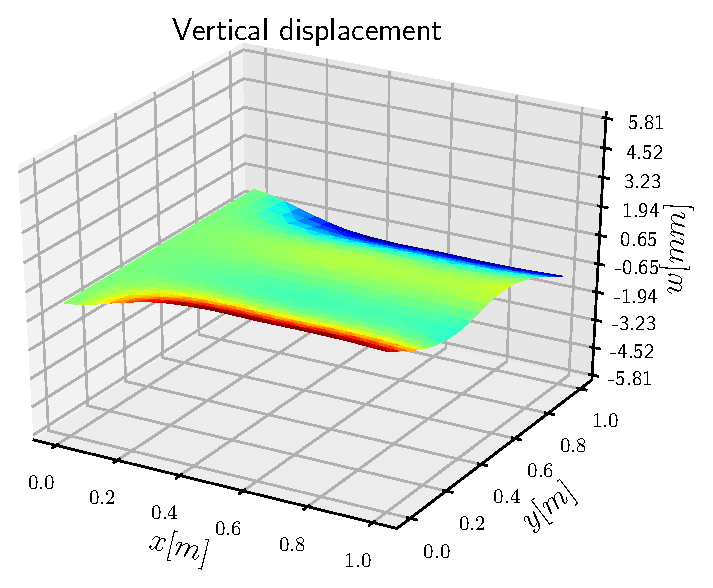
\includegraphics[width=0.45\columnwidth]{Sim1_t_25_cropped.eps}}%
	\hspace{8pt}%
	\subfloat[][$w(t = 0.50 \, t_{\text{fin}})$]{%
		\label{fig:sim1-b}%
		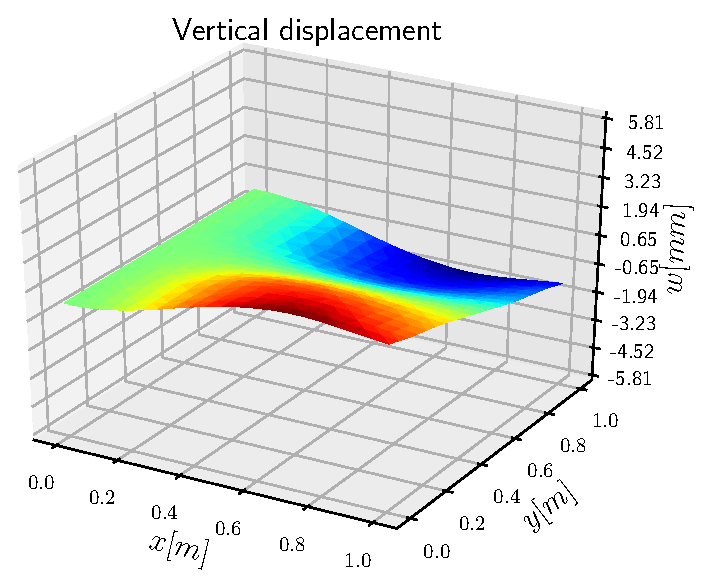
\includegraphics[width=0.45\columnwidth]{Sim1_t_50_cropped.eps}} \\
	\subfloat[][$w(t = 0.75 \, t_{\text{fin}})$]{%
		\label{fig:sim1-c}%
		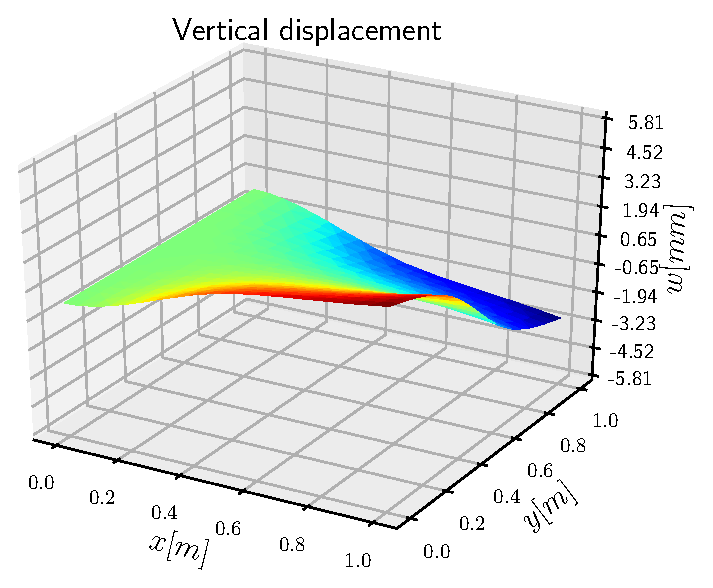
\includegraphics[width=0.45\columnwidth]{Sim1_t_75_cropped.eps}}%
	\hspace{8pt}%
	\subfloat[][$w(t = t_{\text{fin}})$]{%
		\label{fig:sim1-d}%
		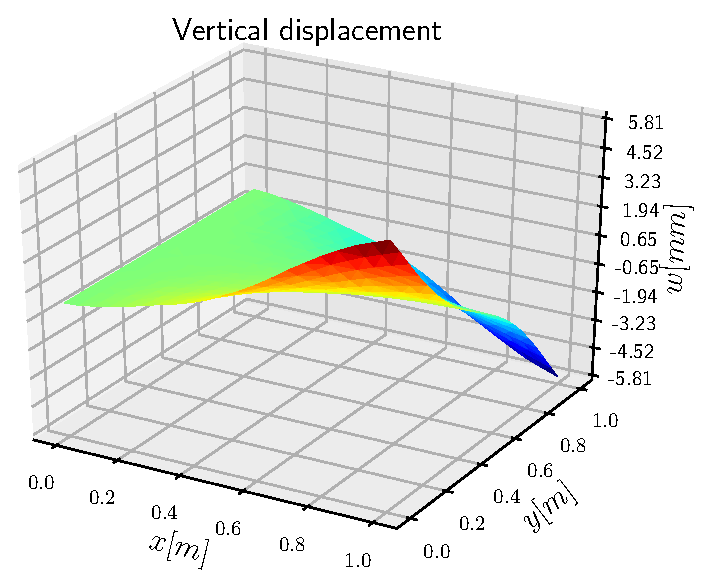
\includegraphics[width=0.45\columnwidth]{Sim1_t_100_cropped.eps}}%
	\caption[Snapshots of the displacement field]{Snapshots for Simulation $n^\circ 1$.}%
	\label{fig:sim1}%
\end{figure}

\begin{figure}[h]%
	\centering
	\subfloat[][$w(t = 0.25 \, t_{\text{fin}})$]{%
		\label{fig:sim2-a}%
		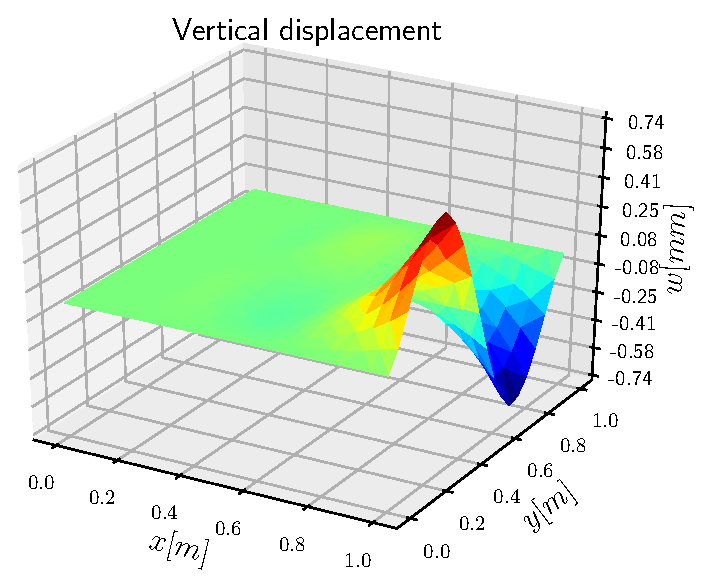
\includegraphics[width=0.45\columnwidth]{Sim2_t_25_cropped.eps}}%
	\hspace{8pt}%
	\subfloat[][$w(t = 0.50 \, t_{\text{fin}})$]{%
		\label{fig:sim2-b}%
		\includegraphics[width=0.45\columnwidth]{Sim2_t_50_cropped.eps}} \\
	\subfloat[][$w(t = 0.75 \, t_{\text{fin}})$]{%
		\label{fig:sim2-c}%
		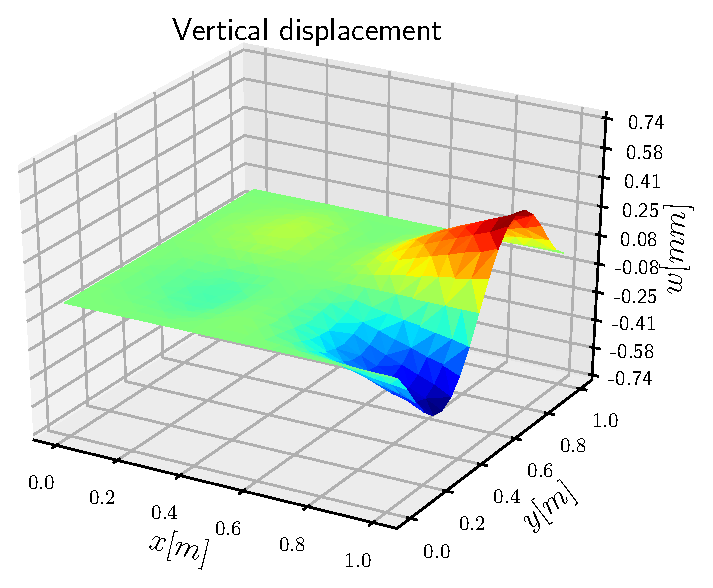
\includegraphics[width=0.45\columnwidth]{Sim2_t_75_cropped.eps}}%
	\hspace{8pt}%
	\subfloat[][$w(t = t_{\text{fin}})$]{%
		\label{fig:sim2-d}%
		\includegraphics[width=0.45\columnwidth]{Sim2_t_100_cropped.eps}}%
	\caption[Snapshots of the displacement field]{Snapshots for Simulation $n^\circ 2$.}%
	\label{fig:sim2}%
\end{figure}

\begin{figure}[h]%
	\centering
	\subfloat[][$w(t = 0.25 \, t_{\text{fin}})$]{%
		\label{fig:sim3-a}%
		\includegraphics[width=0.45\columnwidth]{Sim3_t_25_cropped.eps}}%
	\hspace{8pt}%
	\subfloat[][$w(t = 0.50 \, t_{\text{fin}})$]{%
		\label{fig:sim3-b}%
		\includegraphics[width=0.45\columnwidth]{Sim3_t_50_cropped.eps}} \\
	%\subfloat[][$w(t = 0.75 \, t_{\text{fin}})$]{%
	%	\label{fig:sim3-c}%
	%	\includegraphics[width=0.45\columnwidth]{Sim3_t_75_cropped.eps}}%
	%\hspace{8pt}%
	%\subfloat[][$w(t = t_{\text{fin}})$]{%
	%	\label{fig:sim3-d}%
	%	\includegraphics[width=0.45\columnwidth]{Sim3_t_100_cropped.eps}}%
	\caption[Snapshots of the displacement field]{Snapshots for Simulation $n^\circ 3$}%
	\label{fig:sim3}%
\end{figure}

\begin{figure}[h]%
	\centering
	\subfloat[][Simulation $n^\circ 1$]{%
		\label{fig:sim1-H}%
		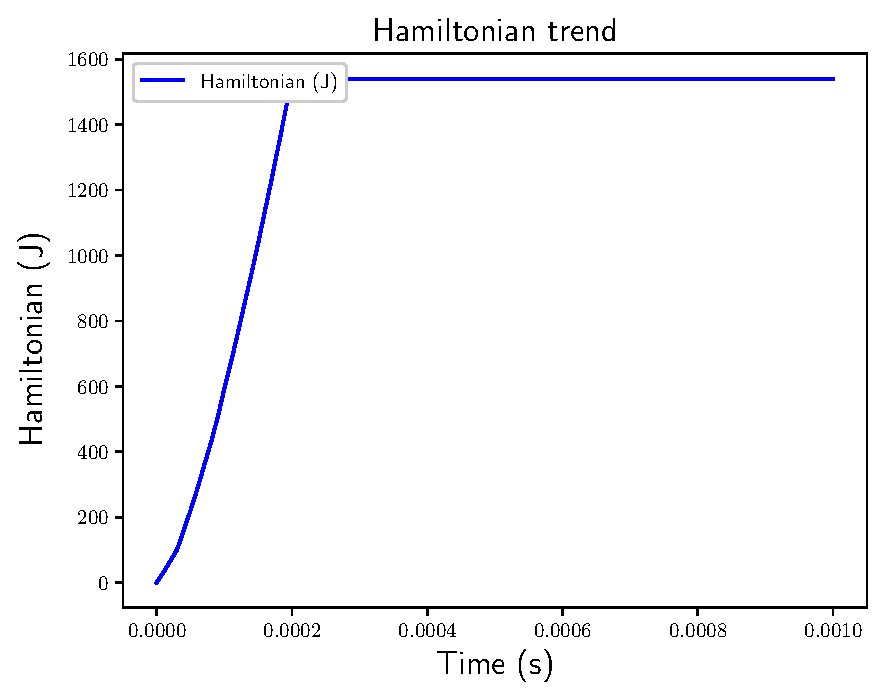
\includegraphics[width=0.45\columnwidth]{Sim1_Hamiltonian_cropped.eps}}%
	\hspace{8pt}%
	\subfloat[][Simulation $n^\circ 2$]{%
		\label{fig:sim2-H}%
		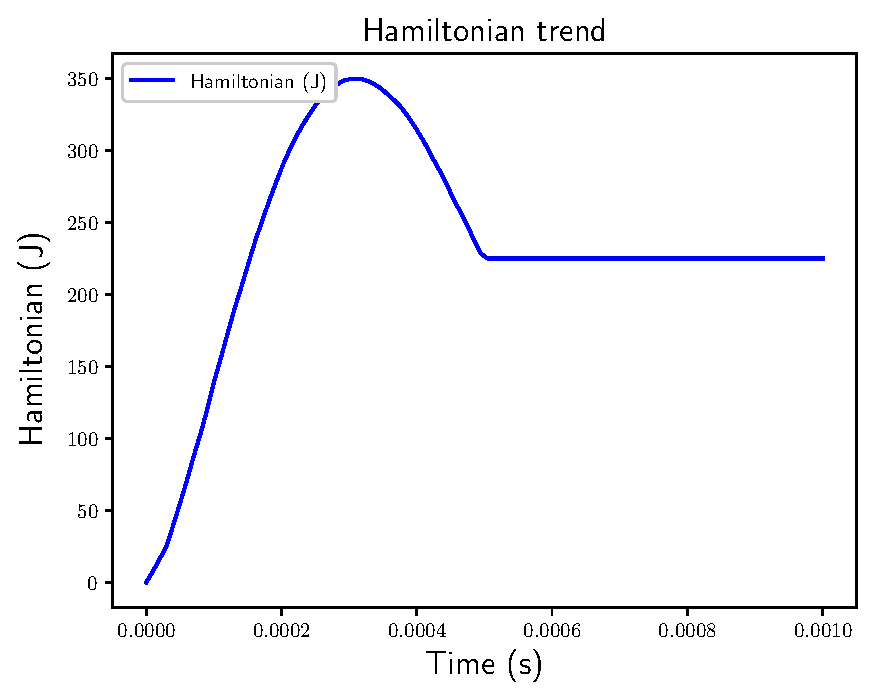
\includegraphics[width=0.45\columnwidth]{Sim2_Hamiltonian_cropped.eps}} \\
	\subfloat[][Simulation $n^\circ 3$]{%
		\label{fig:sim3-H}%
		\includegraphics[width=0.45\columnwidth]{Sim3_Hamiltonian_cropped.eps}} \\
	\caption[Hamiltonian]{Hamiltonian trend for the three simulations.}
	\label{fig:Hamiltonian}
\end{figure}


\section{Conclusion}
This work represents a first attempt to simulate bi-dimensional mechanical systems using the Hamiltonian formalism. The obtained results look convincing, but the model presented herein is not yet fully understood. In particular identifying the proper functional spaces where variables live and the optimal mixed finite element choice is still to be done. Future developments will include the interconnection of this mechanical model with simpler ones, to benefit from the modularity of the port-Hamiltonian framework. Furthermore, to avoid the shear locking phenomenon, the Kirchhoff-Love model will be addressed.

\begin{ack}
The authors would like to thank Michel Sala\"un from ISAE-SUPAERO for the fruitful and insightful discussions.
\end{ack}

\bibliography{biblio_IFACMindlin}             % bib file to produce the bibliography
                                                     % with bibtex (preferred)
                                                   
%\begin{thebibliography}{xx}  % you can also add the bibliography by hand

%\bibitem[Able(1956)]{Abl:56}
%B.C. Able.
%\newblock Nucleic acid content of microscope.
%\newblock \emph{Nature}, 135:\penalty0 7--9, 1956.

%\bibitem[Able et~al.(1954)Able, Tagg, and Rush]{AbTaRu:54}
%B.C. Able, R.A. Tagg, and M.~Rush.
%\newblock Enzyme-catalyzed cellular transanimations.
%\newblock In A.F. Round, editor, \emph{Advances in Enzymology}, volume~2, pages
%  125--247. Academic Press, New York, 3rd edition, 1954.

%\bibitem[Keohane(1958)]{Keo:58}
%R.~Keohane.
%\newblock \emph{Power and Interdependence: World Politics in Transitions}.
%\newblock Little, Brown \& Co., Boston, 1958.

%\bibitem[Powers(1985)]{Pow:85}
%T.~Powers.
%\newblock Is there a way out?
%\newblock \emph{Harpers}, pages 35--47, June 1985.

%\bibitem[Soukhanov(1992)]{Heritage:92}
%A.~H. Soukhanov, editor.
%\newblock \emph{{The American Heritage. Dictionary of the American Language}}.
%\newblock Houghton Mifflin Company, 1992.

%\end{thebibliography}

\appendix

      
                                                          % in the appendices.
\end{document}
